\documentclass[a4paper, 12pt]{article}
\usepackage[UTF8]{ctex}
\usepackage{graphicx}
\usepackage{fancyhdr}
\pagestyle{plain}

\begin{document}

\title{B0.1+B0.2实验报告的撰写}
\author{
  黄雨\\
\small 中山大学
}


\maketitle
\tableofcontents
\newpage

\section{Introduction}

\section{Reference Practice}
\noindent
 This is the first reference cited \cite{WOS:001325770200001}.\\
 This is the second reference cited \cite{WOS:001168307800001}.\\
 This is the third reference cited \cite{WOS:001156734900001}.\\
 This is the fourth reference cited \cite{WOS:001311346600001}.\\
 This is the fifth reference cited \cite{WOS:001183758200001}.\\

\section{Formula Practice}
 \begin{eqnarray}
 \nabla \cdot \mathbf{D} = \rho_f \label{eq:gauss_electric} \\
 \nabla \cdot \mathbf{B} = 0 \label{eq:gauss_magnetic} \\
 \nabla \times \mathbf{E} = -\frac{\partial \mathbf{B}}{\partial t} \label{eq:faraday} \\
 \nabla \times \mathbf{H} = \mathbf{J}_f + \frac{\partial \mathbf{D}}{\partial t} \label{eq:ampere_maxwell}\\
 E = mc^2\label{eq:einstein}\\
 \end{eqnarray}

 \newpage
 \section{Inserting Images}
  \begin{figure}[h] 
    \centering
    
\includegraphics[width=0.3\textwidth]{Figure1.png} 
    \caption{彩色位图}
    \label{Figure 1} 
  \end{figure}
  \begin{figure}[h]
    \centering
    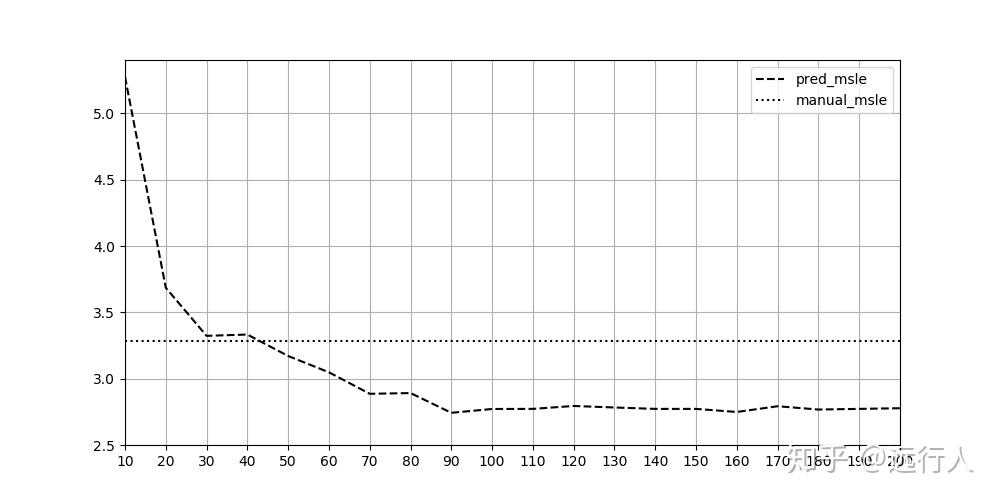
\includegraphics[width=0.8\textwidth]{Figure2.jpg} 
    \caption{黑白曲线图}
    \label{Figure 2} 
  \end{figure}

\newpage
\section{Inserting Tables}
 \begin{table}[h]
  \centering
  \begin{tabular}{|l|l|}
  Apples       & Green  \\
  Strawberries & Red    \\
  Orange       & Orange \\
  \end{tabular}
 \label{Table}
 \caption{表格}
 \end{table}

\section{Reference}
 \bibliographystyle{unsrt} 
 \bibliography{savedrecs} 

\end{document}
